\chapter{Uniform Plane Wave in an arbitrary direction}\label{lec:lec29}

Prior to now, we have discussed  plane wave propagation has been in an unbound medium, orienting our co-ordinate system such that the wave propagated was in the direction of one of the axis(the z-axis).This was done because an unbound medium is symmetric in all directions, regardless of the direction looked from the medium appears same.
However, in a bound medium, the co-ordinate axis choice might affect the analysis algebraically.
Essentially we select a co-ordinate system that will enable our analysis be simple, doing this restricts the choice of co-ordinate axis. First we would investigate the propagation of electro-magnetic waves in a semi-finite medium (i.e half of an unbound medium), then move on to bound medium. However before this analysis we require a representation of electro-magnetic wave traveling in an arbitrary direction with respect to the co-ordinate axis.
\begin{figure}[h]
\centering
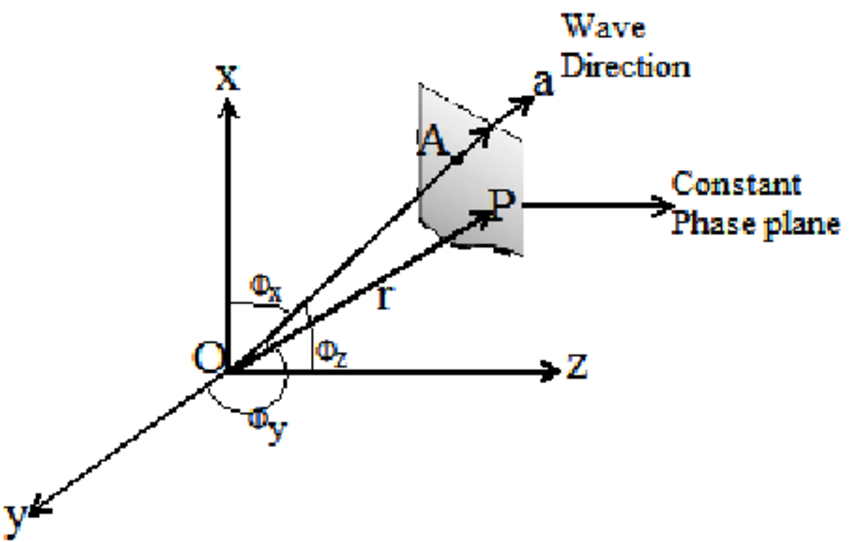
\includegraphics[scale=0.3]{\pathtopartone/graphics/em-waves}
\caption{wave in arbitrary direction}
\end{figure}

\section{Wave in arbitrary direction}
Recall when we had a co-ordinate system such that the wave was propagating in the z-axis, it's phase variation was also in the same direction while it's electric and magnetic fields were in planes perpendicular to the z-axis(i.e the x-y plane).
Say we have an unbound medium, the wave would still be oriented such that it is moving in an arbitrary direction with respect to the co-ordinate axis.

In fig(29.1) a wave propagation in an arbitrary direction is shown; a constant phase plane(i.e the plane which the electric and magnetic field lie) is shown perpendicular to the waves direction.
$\phi_{x}$,$\phi_{y}$ and $\phi_{z}$ are the angles which the wave makes with the x, y and z axis respectively. 
The vector has direction cosines $\cos\phi_{x}\hat{x}$, $\cos\phi_{y}\hat{y}$, $\cos\phi_{z}\hat{z}$. The unit vector:
\begin{equation}
\hat{n} = \cos\phi_{x}\hat{x} + \cos\phi_{y}\hat{y} + \cos\phi_{z}\hat{z}
\end{equation}

Taking two arbitrary points on the wave direction point O and P, where O is the origin and P has co-ordinates (x,y,z).

Thus $\vec{OP}$ = $x\hat{x}$ + $y\hat{y}$ + $z\hat{z}$

The normal distance to take to any point on the constant phase plane is OA , so if any point is taken on the plane and it's projection is found in the direction of the normal, the quantity is fixed regardless of the point it is taking on the phase plane.

The equation of the phase plane will be:

\begin{center}
$\hat{n}$.$\vec{OP}$ (i.e the dot product of $\hat{n}$ and $\vec{OP}$)

$\hat{n}$.$\vec{OP}$ = $\left|OA \right|$  = constant

substituting for $\hat{n}$ and $\vec{OP}$
\end{center}
$x\cos\phi_{x}$ + $y\cos\phi_{y}$ + $z\cos\phi_{z}$ = constant
Since, the magnitude of $\vec{OA}$ is constant that tells us the distance of the plane from its origin.

if $\beta$ is the phase constant and distance $\vec{OA}$ the phase of the plane is $\beta$ multiplied by the distance traveled which is $\vec{OA}$.

\begin{center}
therefore, Phase of the plane = $\beta$ $\left|OA \right|$ = $\beta$ $\hat{n}.\hat{r}$

where $\hat{r}$ = $\vec{OP}$ = $x\hat{x}$ + $y\hat{y}$ + $z\hat{z}$

\end{center}
$\beta$ = Phase constant,
$\hat{n}$ = Unit vector in the direction of propagated wave,
$\hat{r}$ = Position of any Vector on the constant phase plane

Since we have the phase plane, the expression of electric and magnetic field which corresponds to the wave propagation is straight forward
\begin{center}

Electric field $\bar{E}$ = $\bar{E}_{0}e^{-j\beta \hat{n}.\hat{r}}$

\end{center}
$\bar{E}_{0}.\hat{n} = 0$

Since $\bar{E}_{0}$ is perpendicular to $\hat{n}$,
$\bar{E}_{0}$ = Magnitude of the Vector,
$-j\beta \hat{n}.\hat{r}$ = Phase Variation.

therefore, $\bar{E}$ = $\bar{E}_{0}e^{-j\beta \hat{n}.\hat{r}}$ represents an electromagnetic wave traveling in an arbitrary direction $\hat{n}$.
Combining $\beta\hat{n}$ we define another vector called the wave vector.

wave vector $\bar{k} \equiv \beta \hat{n}$ = $\beta(\cos\phi_{x}\hat{x} + \cos\phi_{y}\hat{y} + \cos\phi_{z}\hat{z})$
\begin{center}
$\bar{k}$ = $\beta\cos\phi_{x}\hat{x}$ + $\beta\cos\phi_{y}\hat{y}$ + $\beta\cos\phi_{z}\hat{z}$
\end{center}
Let $K_{x}$ = $\beta\cos\phi_{x}$, $K_{y}$ = $\beta\cos\phi_{y}$, 
$K_{z}$ = $\beta\cos\phi_{z}$

$\bar{k}$ = $K_{x}\hat{x}$ + $K_{y}\hat{y}$ + $K_{z}\hat{z}$

So if the direction of wave propagation($\hat{n}$) and phase constant($\beta$) which depend on the medium parameters are known, then we can define $\bar{k}$ which completely characterizes the wave in the arbitrary direction.

Recall $\hat{E}_{0}.\hat{n}$ = 0 since they are perpendicular, then
\begin{center}
$\hat{E}\cdot k$ = 0
\end{center}
Therefore, to verify if the wave is traveling in the z-direction then
\begin{center}
$\phi_{z}$ = 0, $\phi_{y}$ = 90\textdegree, $\phi_{x}$ = 90\textdegree
Therefore, $\bar{k}$ = $\beta(\cos90\hat{x} + \cos90\hat{y} + \cos0\hat{z})$

$\hat{k}$ = $\beta.\hat{z}$

Therefore, space variation = $e^{-j\beta z}$
\end{center}
This is the same expression we got for a wave which was traveling in the z direction.
\\Therefore,

$\hat{E}$ = $\hat{E}_{0} e^{-j\beta\hat{n}.\hat{r}}$ is a representation of the electric for a uniform plane wave traveling in an arbitrary direction making angles $\phi_{x}$, $\phi_{y}$ and $\phi_{z}$ with the three co-ordinate axes.


To find the magnetic field corresponding to the electric field, we go back to the original Maxwell's equation.

Since we are still dealing with the media which does not have conductivity, we say let's have a source free media i.e no conductivity or currents.

The Maxwell's equation:

\begin{equation}
\bigtriangledown\times\bar{H} = j\omega\epsilon\bar{E}
\end{equation}
\begin{equation}
\bigtriangledown\times\bar{E} = -j\omega\mu\bar{H}
\end{equation}

\begin{equation}
\hat{H} = \frac{-1}{j\omega\mu}(\bigtriangledown\times\bar{E}) = 
\frac{-1}{j\omega\mu}
\end{equation}

\[ 
\begin{vmatrix}
$$\hat{x}$$ & $$\hat{y}$$ & $$\hat{z}$$\\
$$\frac{\partial}{\partial x}$$ x & $$\frac{\partial}{\partial y}$$ & $$\frac{\partial}{\partial z}$$\\
$$E_{x}$$ & $$E_{y}$$ & $$E_{z}$$
\end{vmatrix}
\]
\newline
The electric field vector $\hat{E}$ can be determined explicitly in it's component as:

\begin{align}
\bar{E} = [E_{0x}\hat{x} + E_{0y}\hat{y} + E_{0z}\hat{z}]^{-j\bar{k}.\bar{r}}
\end{align}

Note that, $E_{0x}$, $E_{0y}$ and $E_{0z}$ are not functions of the space since the electric field is constant everywhere in the space, hence space variation is only present in $e^{-j\bar{k}.\bar{r}}$.
So taking a component and it's derivative w.r.t x will be:

\begin{equation}
\frac{\delta}{\delta x} [E_x,E_y,E_z] = -jk_x[E_x,E_y,E_z]
\end{equation}

This means $\frac{\delta}{\delta x}$ = $-jk_x$, $\frac{\delta}{\delta y}$ = $-jk_y$ 
and $\frac{\delta}{\delta z}$ = $-jk_z$.
Therefore, substituting for $\frac{\delta}{\delta x}$, $\frac{\delta}{\delta y}$ and $\frac{\delta}{\delta z}$ into equation(29.4) we get:
\begin{equation}
\hat{H} = 
\begin{vmatrix}
\hat{x} & \hat{y} & \hat{z}\\
-jk_x & -jk_y & -jk_z\\
E_{x} & E_{y} & E_{z}
\end{vmatrix}
\end{equation}

But, since this quantity is a cross product of $-jk$ and $E$ it can be written as:
\begin{equation}
\frac{-1}{j\omega\mu} [-j\bar{k}\times\bar{E}] = \frac{1}{\omega\mu} \bar{k}\times\bar{E}
\end{equation}

$k$ = direction of wave propagation.
$E$ = direction of the electric field.
$\bar{H}$ = cross product of $k$ and $E$, meaning it is perpendicular to both.

Say we have a wave traveling in an arbitrary direction with electric field:
\begin{equation}
\bar{E} = E_0 e^{-j\bar{k}.\bar{r}} = \bar{E}_0[e^{(-j\beta\cos\phi_{x}x + \beta\cos\phi_{y}y + \beta\cos\phi_{z}z)}]
\end{equation}

Considering only the space space variation the z-direction:
\begin{equation}
\bar{E} = \bar{E}_0 e^{-j\beta(\cos\phi_{x}x + \cos\phi_{y}y)}.e^{-j\beta(\cos\phi_{z}z)}
\end{equation}

Note that if we move in the x-y plane we have a phase variation which means the x-y plane is not a constant phase plane, this is visible from fig.1. But there is a variation in the z-direction.

So looking at the wave, what is the variety with which the phase point moves in the z-direction?

So we take the phase in the direction of z.The effective phase constant which the wave sees in the z-direction is $\beta\cos\phi_{z}z$.

Wave phase constant in z-direction($\beta z$):
\begin{equation}
\beta z = \beta\cos\phi_{z}
\end{equation}
Phase velocity in the z-direction:
\begin{equation}
v_{pz} = \frac{\omega}{\beta_z} = \frac{\omega}{\beta\cos\phi_{z}}
\end{equation}
But $\frac{\omega}{\beta}$ is the velocity of the wave in the direction of the wave propagation.

\begin{equation}
\frac{\omega}{\beta}\times \frac{1}{\cos\phi_{z}} = \frac{v_0}{\cos\phi_{z}}
\end{equation}

Therefore, $v_0$ is the velocity of the wave in the direction perpendicular to the phase i.e the wave velocity in an unbound medium.

But the phase velocity of the wave in the z-direction is $\frac{v_0}{\cos\phi_{z}}$.

We can also have the phase velocity velocities in other directions:
\begin{center}
$\beta_x = \beta\cos\phi_{x}$, $\beta_y = \beta\cos\phi_{y}$\\
$v_px$ = $\frac{\omega}{\beta_x}$ = $\frac{\omega}{\beta\cos\phi_{x}}$ = $\frac{v_0}{\cos\phi_{x}}$\\
$v_py$ = $\frac{\omega}{\beta_y}$ = $\frac{\omega}{\beta\cos\phi_{y}}$ = $\frac{v_0}{\cos\phi_{y}}$
\end{center}
Since $\cos\phi_{x}$, $\cos\phi_{y}$ and $\cos\phi_{z}$ are always less than 1, $v_p$ is always greater than $v_0$(intrinsic velocity).
\begin{center}
$v_px$, $v_py$, $v_pz$ $\geq$ $v_0$
also when $\phi_{x}$, $\phi_{y}$, or $\phi_{z}$ = 0, $v_p$ = $\infty$
therefore, $\infty$ $\geq$ $v_px$, $v_py$, $v_pz$ $\geq$ $v_0$
\end{center}
Since we are talking about velocities greater than the intrinsic velocities, we know light is an electro-magnetic wave. And we know the intrinsic velocity of light will be the velocity of light $C$ i.e $v_0 = C$.
But from physics we know that the velocity of any system can not be greater than the velocity of light.
Does that mean we have found a mechanism that can transfer energy faster than the speed of light?
No. This is because this velocity is not the velocity of any energy packet or physical point in space because the wave defines its velocity which is based on the phase fronts. This essentially gives the condition that $v_p$ $<$ $v_0$.

Re-examining it:
\begin{figure}[h]
\centering
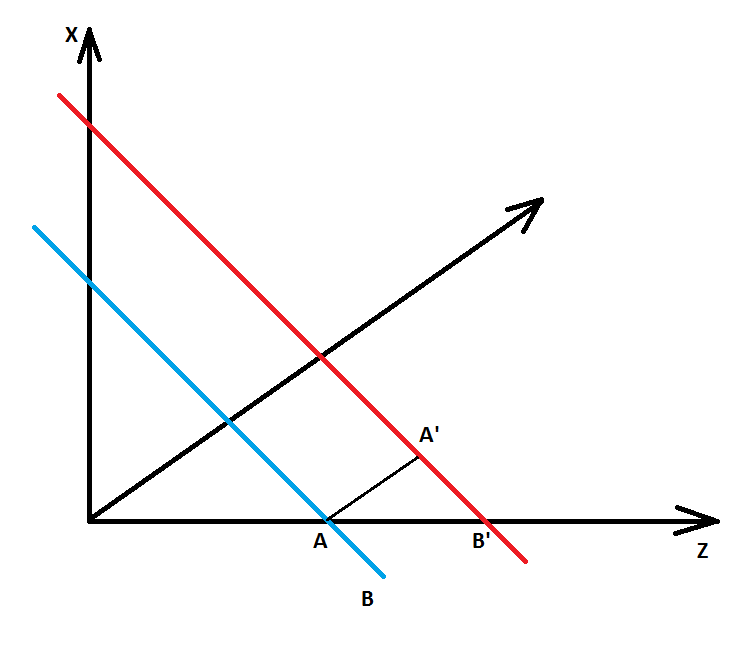
\includegraphics[width=.6\linewidth]{\pathtopartone/graphics/img2}
\caption{}
\end{figure}

From fig(29.2) we have a wave traveling in the x-z plane, with the constant wave fronts shown, by the time the wave travels between two points on its axis, the constant phase points (given by the entire phase fronts) moves between two points(A and B'), unless the wave is parallel to the constant wave fronts the distance moved by the front is always greater than that of the wave, while that happened the point A has not moved to the point B', rather it has measured from A to A', so the point that moved to B' was not A but rather it was from point B which has now moved to B'. So when the wave is moving a defined point (A) on the wave front it only moves by a distance AA', however when measuring the phase velocities we simply measure the separation between the points on the z-axis and ask how much time was spent changing positions. So essentially we measure the distance, find how much phase change it has undergone and from there we can get the phase velocity.

So from this we can see that the phase velocity is not really giving us the velocity of a particular point on the phase line. In fact when we define the phase velocity the entire constant phase plane is behaving like a point, so we just take two points (but both points are representing the same phase) so if we find the same phase we say the distance with a constant phase point has moved from the first to the second point, this is the reason we get the velocity of a particular point on the phase front.

So the velocity, AB (whatever phase velocity we get) is not simply the the resolution of the velocity vector in 3-directions, because resolving the velocity in 3-directions will always make it less than the actual velocity but in this case we see that the components of the phase velocity in three directions $v_px$, $v_py$ and $v_pz$ are always greater than the velocity vector, so this is not a simple vector resolution of the velocity of the wave, in fact the phase velocities are calculated from the distance traveled by the constant phase point along the z-axis and that gives the velocity:
\begin{dmath*}
\frac{\text{Intrinsic Velocity}}{\text{Direction Cosines}}
\end{dmath*}
So as the wave become more and more perpendicular to the z-axis: meaning moving in the x direction, the phase front becomes parallel to the z-axis, at point A a small tilt shows that the point is moving very rapidly. So by a small tilt it would have moved by a large distance in the z-direction, that is the point has moved a small distance in the x-axis when the phase front is almost parallel to the z-axis, so what we find is that if the wave was moving along the x-axis and if the phase fronts were parallel to the z-axis, then a small movement of the wave the point moves by by a very large distance. And if the wave was perfectly parallel to the z-axis the point moves from $-\infty$ to +$\infty$ even for infinitesimal movement of the wave in the x-direction.

So when the phase velocity approaches infinity the wave move in the x-direction, so that the point vector for the wave is in the x-direction, there is no point moving in the z-direction.
As the phase velocity approaches infinity we might ask with what velocity does the energy travel in the z-direction.
So in general we might ask a question if the wave is moving with a velocity $v_p$ in the z-direction, with what velocity is the energy moving in the z-direction.
And we say that the velocity in the AB' direction which is $v_0$ will be $v_0\times\cos\phi_{z}$, so the velocity with which the point A moves in the z-direction will be $v_0\cos\phi_{z}$ and if it is in the x-direction it will be $v_0\cos\phi_{x}$. So the velocity with which a given point on the phase front moves in the z-direction is called the \textbf{group velocity($v_g$)}

\begin{center}
Group velocity in the z-direction $v_gz$ :
$v_gz$ = $v_0\cos\phi_{z}$
\end{center}
So since $\cos\phi_{z} < 1$, $v_g$(which is the velocity of a particular point)$\leq v_0$


Group velocity in the following:
\begin{enumerate}[(i)]
\item x-direction:	$v_{gx}$ = $v_0\cos\phi_{x}$
\item y-direction: 	$v_{gy}$ = $v_0\cos\phi_{y}$
\item z-direction:	$v_{gz}$ = $v_0\cos\phi_{z}$
\end{enumerate}
$0\leq v_{gx},v_{gy},v_{gz}$ $\leq$ $v_0$ but recall, $\infty\geq v_{gx},v_{gy},v_{gz}$ $\geq$ $v_0$

From this we can see that the $v_p$ never goes below $v_0$ and $v_g$ never goes above $v_0$,
So we have a kind of dividing line:
\begin{figure}[h]
\centering
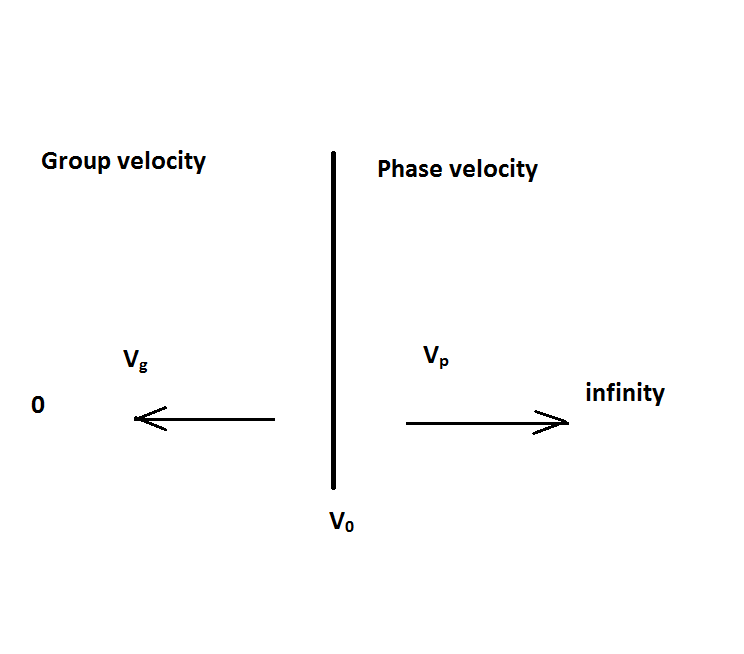
\includegraphics[width=.6\linewidth]{\pathtopartone/graphics/img3}
\caption{}
\end{figure}

Only in a situation where the wave is traveling in the x,y,z direction or if we find the velocity of the wave both $v_p$ and $v_g$ in the direction of wave motion then both $v_p$ and $v_p$ will be $v_{0}^2$.
\begin{equation}
v_D v_g = v_{0}^2
\end{equation}
So taking $v_D$ and $v_g$ in the same direction their product is $v_{0}^2$, this means that when $v_p$ approaches infinity the product of $v_p$ and $v_g$ is constant i.e $v_{0}^2$.

So as $v_p$ increases $v_g$ reduces. So when calculating the speed of energy flow we find $v_g$, but when we talk of the moment of phase in the medium the velocity is given as the phase velocity.

Wavelength in the following:
\begin{enumerate}[(i)]
\item x-direction: 
\begin{dmath*}	
\frac{v_{px}}{f} = \frac{v_0/\cos\phi_{x}}{f}
= \frac{\lambda_0}{\cos\phi_{x}}
\end{dmath*}
\item y-direction: 	
\begin{dmath*}
\frac{v_{py}}{f} = \frac{v_0/\cos\phi_{y}}{f}
= \frac{\lambda_0}{\cos\phi_{y}}
\end{dmath*}
\item z-direction: 	
\begin{dmath*}
\frac{v_{pz}}{f} = \frac{v_0/\cos\phi_{z}}{f}
= \frac{\lambda_0}{\cos\phi_{z}}
\end{dmath*}
\end{enumerate}